\section{Approach}\label{sec:approach}

\subsection{Scope of the work}

In this work, it is intended to reproduce the method proposed by the original Netflix attack. Hence, \autoref{alg:algo} has been implemented in Python, using the scoring metric defined by \autoref{eq:score}.

However, several differences with the original paper are to be highlighted. Firstly, it used 50 records from the IMDb. However, the datasets that are currently publicly available from the IMDb are the ratings for each movie, but not the ratings from a given user. A solution would be to get this data directly from the IMDb website because the ratings of a user are public if he also wrote a review. A data miner that parses the content of random IMDb users could do the job, but there are two obstacles:

\begin{itemize}
	\item it would be of significant complexity, and is out of scope of the project.
	\item the terms and conditions of IMDb prohibit the usage of "data mining, robots, screen scraping, or similar data gathering and extraction tools”\footnote{see \url{https://www.imdb.com/conditions}}. It can be suspected that it is the reason only 50 entries we used in the original attack. 
\end{itemize}

As a workaround, it is proposed to use the MovieLens dataset as auxiliary information. MovieLens is a web-based movie recommender system that makes its database available for research \cite{movielens-db}. This database has already been used in privacy-related research, such as \cite{movielens}. As opposed to the IMDb case, the "anonymous" user IDs are consistent across all the movie ratings that are registered, which makes it suitable for the user re-identification. Also, it is the occasion to test another dataset against the Netflix one.

After the raw implementation of the matching algorithm, a verification procedure is proposed to assess its robustness. Indeed, it is needed to validate the algorithm without knowing the ground truth of the matching users.  

\subsection{Data pre-processing}

A significant amount of pre-processing was needed on both the MovieLens and Netflix datasets before being able to run the matching algorithm. 

On one hand, the Netflix dataset contains over 100 million ratings from 480,000 users (around 5.5 \si{\giga\byte} of data). One folder contains 17,770 files (one per movie) filled with three columns: \texttt{userID, rating, date}. Another file maps each file to a movie name and specifies the movie release date. On the other hand, the MovieLens database has a different structure. It contains one file filled with four columns: \texttt{userID, movieID, rating, timestamp} as well a file mapping movieIDs to titles. \autoref{fig:nf-struct} depicts how the Netflix dataset was processed to give it the same structure as the MovieLens one.

\begin{figure}[h]
	\centering
	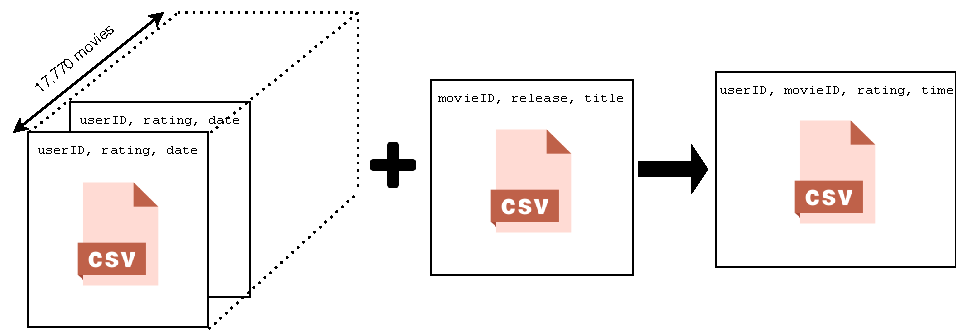
\includegraphics[width=\linewidth]{img/processing.pdf}
	\caption{Data reshaping of the Netflix dataset.}
	\label{fig:nf-struct}
\end{figure}

After the reshaping process, useless entries from both database were removed to make the score computation faster later on. Entries can be discarded for different reasons:

\begin{itemize}
	\item Out-of-bounds timestamps: according to its ReadMe, the MovieLens database has records from ratings performed between January 09, 1995 and March 31, 2015. The Netflix database only ranges from October 1998 to December 2005, so that many ratings can be eliminated. The amount of distinct users from MovieLens drops from 138,493 to 52,875.
	
	\item Isolated movie: a movie rating is removed from one database if it is not present in the other database. (it would not be taken into account in the scoring function anyway). A movie was identified by its title and release date to filter only those appearing in both datasets\footnote{Few special cases were also discarded, for example the fact that two movies named \textit{Hamlet} were released in 2000, so that it was not possible to differentiate between them.}. There were around 5800 movies that were rated in both datasets (from the original 17,700 of Netflix).
\end{itemize}

Ultimately, the movie IDs needed to be made consistent between the two datasets to allow for proper implementation of the scoring function. Indeed, movies were not given the same \texttt{movieID} in both datasets.

Those lengthy data manipulations are not de-anonymization \textit{per se} but are an unavoidable step needed to allow the implementation of the algorithm.